%% LyX 2.3.2 created this file.  For more info, see http://www.lyx.org/.
%% Do not edit unless you really know what you are doing.
\documentclass[english,aspectratio=169, handout]{beamer}
\usepackage{mathptmx}
\usepackage{eulervm}
\usepackage[T1]{fontenc}
\usepackage[latin9]{inputenc}
\usepackage{babel}
\usepackage{amsmath}
\usepackage{amssymb}
\usepackage{graphicx}
\ifx\hypersetup\undefined
  \AtBeginDocument{%
    \hypersetup{unicode=true,pdfusetitle,
 bookmarks=true,bookmarksnumbered=false,bookmarksopen=false,
 breaklinks=false,pdfborder={0 0 0},pdfborderstyle={},backref=false,colorlinks=true,
 allcolors=NYUPurple,urlcolor=LightPurple}
  }
\else
  \hypersetup{unicode=true,pdfusetitle,
 bookmarks=true,bookmarksnumbered=false,bookmarksopen=false,
 breaklinks=false,pdfborder={0 0 0},pdfborderstyle={},backref=false,colorlinks=true,
 allcolors=NYUPurple,urlcolor=LightPurple}
\fi

\makeatletter

%%%%%%%%%%%%%%%%%%%%%%%%%%%%%% LyX specific LaTeX commands.
%% A simple dot to overcome graphicx limitations
\newcommand{\lyxdot}{.}


%%%%%%%%%%%%%%%%%%%%%%%%%%%%%% Textclass specific LaTeX commands.
% this default might be overridden by plain title style
\newcommand\makebeamertitle{\frame{\maketitle}}%
% (ERT) argument for the TOC
\AtBeginDocument{%
  \let\origtableofcontents=\tableofcontents
  \def\tableofcontents{\@ifnextchar[{\origtableofcontents}{\gobbletableofcontents}}
  \def\gobbletableofcontents#1{\origtableofcontents}
}

%%%%%%%%%%%%%%%%%%%%%%%%%%%%%% User specified LaTeX commands.
\usetheme{CambridgeUS} 
\beamertemplatenavigationsymbolsempty


% Set Color ==============================
\definecolor{NYUPurple}{RGB}{87,6,140}
\definecolor{LightPurple}{RGB}{165,11,255}


\setbeamercolor{title}{fg=NYUPurple}
%\setbeamercolor{frametitle}{fg=NYUPurple}
\setbeamercolor{frametitle}{fg=NYUPurple}

\setbeamercolor{background canvas}{fg=NYUPurple, bg=white}
\setbeamercolor{background}{fg=black, bg=NYUPurple}

\setbeamercolor{palette primary}{fg=black, bg=gray!30!white}
\setbeamercolor{palette secondary}{fg=black, bg=gray!20!white}
\setbeamercolor{palette tertiary}{fg=gray!20!white, bg=NYUPurple}

\setbeamertemplate{headline}{}

\setbeamercolor{parttitle}{fg=NYUPurple}
\setbeamercolor{sectiontitle}{fg=NYUPurple}
\setbeamercolor{sectionname}{fg=NYUPurple}
\setbeamercolor{section page}{fg=NYUPurple}

\AtBeginSection[]{
  \begin{frame}
  \vfill
  \centering
\setbeamercolor{section title}{fg=NYUPurple}
 \begin{beamercolorbox}[sep=8pt,center,shadow=true,rounded=true]{title}
    \usebeamerfont{title}\usebeamercolor[fg]{title}\insertsectionhead\par%
  \end{beamercolorbox}
  \vfill
  \end{frame}
}

\makeatother

\begin{document}
\global\long\def\reals{\mathbf{R}}%
 
\global\long\def\integers{\mathbf{Z}}%
 
\global\long\def\naturals{\mathbf{N}}%
 
\global\long\def\rationals{\mathbf{Q}}%
 
\global\long\def\ca{\mathcal{A}}%
 
\global\long\def\cb{\mathcal{B}}%
 
\global\long\def\cc{\mathcal{C}}%
 
\global\long\def\cd{\mathcal{D}}%
 
\global\long\def\ce{\mathcal{E}}%
 
\global\long\def\cf{\mathcal{F}}%
 
\global\long\def\cg{\mathcal{G}}%
 
\global\long\def\ch{\mathcal{H}}%
 
\global\long\def\ci{\mathcal{I}}%
 
\global\long\def\cj{\mathcal{J}}%
 
\global\long\def\ck{\mathcal{K}}%
 
\global\long\def\cl{\mathcal{L}}%
 
\global\long\def\cm{\mathcal{M}}%
 
\global\long\def\cn{\mathcal{N}}%
 
\global\long\def\co{\mathcal{O}}%
 
\global\long\def\cp{\mathcal{P}}%
 
\global\long\def\cq{\mathcal{Q}}%
 
\global\long\def\calr{\mathcal{R}}%
 
\global\long\def\cs{\mathcal{S}}%
 
\global\long\def\ct{\mathcal{T}}%
 
\global\long\def\cu{\mathcal{U}}%
 
\global\long\def\cv{\mathcal{V}}%
 
\global\long\def\cw{\mathcal{W}}%
 
\global\long\def\cx{\mathcal{X}}%
 
\global\long\def\cy{\mathcal{Y}}%
 
\global\long\def\cz{\mathcal{Z}}%
 
\global\long\def\ind#1{1(#1)}%
 %\newcommand{\pr}{P}
\global\long\def\pr{\mathbb{P}}%
 
\global\long\def\predsp{\cy}%
 %{\hat{\cy}}
\global\long\def\outsp{\cy}%

\global\long\def\prxy{P_{\cx\times\cy}}%
 
\global\long\def\prx{P_{\cx}}%
 
\global\long\def\prygivenx{P_{\cy\mid\cx}}%
 %\newcommand{\ex}{E}
\global\long\def\ex{\mathbb{E}}%
 
\global\long\def\var{\textrm{Var}}%
 
\global\long\def\cov{\textrm{Cov}}%
 
\global\long\def\sgn{\textrm{sgn}}%
 
\global\long\def\sign{\textrm{sign}}%
 
\global\long\def\kl{\textrm{KL}}%
 
\global\long\def\law{\mathcal{L}}%
 
\global\long\def\eps{\varepsilon}%
 
\global\long\def\as{\textrm{ a.s.}}%
 
\global\long\def\io{\textrm{ i.o.}}%
 
\global\long\def\ev{\textrm{ ev.}}%
 
\global\long\def\convd{\stackrel{d}{\to}}%
 
\global\long\def\eqd{\stackrel{d}{=}}%
 
\global\long\def\del{\nabla}%
 
\global\long\def\loss{\ell}%
 
\global\long\def\risk{R}%
 
\global\long\def\emprisk{\hat{R}}%
 
\global\long\def\lossfnl{L}%
 
\global\long\def\emplossfnl{\hat{L}}%
 
\global\long\def\empminimizer#1{\hat{#1}^{*}}%
 
\global\long\def\minimizer#1{#1^{*}}%
\global\long\def\optimizer#1{#1^{*}}%
 
\global\long\def\etal{\textrm{et. al.}}%
 
\global\long\def\tr{\operatorname{tr}}%

\global\long\def\trace{\operatorname{trace}}%
 
\global\long\def\diag{\text{diag}}%
 
\global\long\def\rank{\text{rank}}%
 
\global\long\def\linspan{\text{span}}%
 
\global\long\def\spn{\text{span}}%
 
\global\long\def\proj{\text{Proj}}%
 
\global\long\def\argmax{\operatornamewithlimits{arg\, max}}%
 
\global\long\def\argmin{\operatornamewithlimits{arg\, min}}%

\global\long\def\bfx{\mathbf{x}}%
 
\global\long\def\bfy{\mathbf{y}}%
 
\global\long\def\bfl{\mathbf{\lambda}}%
 
\global\long\def\bfm{\mathbf{\mu}}%
 
\global\long\def\calL{\mathcal{L}}%

\global\long\def\vw{\boldsymbol{w}}%
 
\global\long\def\vx{\boldsymbol{x}}%
 
\global\long\def\vxi{\boldsymbol{\xi}}%
 
\global\long\def\valpha{\boldsymbol{\alpha}}%
 
\global\long\def\vbeta{\boldsymbol{\beta}}%
 
\global\long\def\vsigma{\boldsymbol{\sigma}}%
\global\long\def\vtheta{\boldsymbol{\theta}}%
 
\global\long\def\vd{\boldsymbol{d}}%
 
\global\long\def\vs{\boldsymbol{s}}%
 
\global\long\def\vt{\boldsymbol{t}}%
 
\global\long\def\vh{\boldsymbol{h}}%
 
\global\long\def\ve{\boldsymbol{e}}%
 
\global\long\def\vf{\boldsymbol{f}}%
 
\global\long\def\vg{\boldsymbol{g}}%
 
\global\long\def\vz{\boldsymbol{z}}%
 
\global\long\def\vk{\boldsymbol{k}}%
 
\global\long\def\va{\boldsymbol{a}}%
 
\global\long\def\vb{\boldsymbol{b}}%
 
\global\long\def\vv{\boldsymbol{v}}%
 
\global\long\def\vy{\boldsymbol{y}}%

\global\long\def\dom{\textrm{\textbf{dom} }}%
\global\long\def\rank{\text{\textbf{rank }}}%
\global\long\def\conv{\textrm{\textbf{conv} }}%
\global\long\def\relint{\text{\textbf{relint }}}%
\global\long\def\aff{\text{\textbf{aff }}}%

\global\long\def\hil{\ch}%
 
\global\long\def\rkhs{\hil}%
 
\global\long\def\ber{\text{Ber}}%

\title[DS-GA 1003 / CSCI-GA 2567]{Subgradient Descent}
\author{Xintian Han \& David S. Rosenberg }
\date{Feb 13, 2019}
\institute{NYU CDS}

\makebeamertitle
\mode<article>{Just in article version}

\begin{frame}{Contents}
\tableofcontents{}
\end{frame}


\section{Motivation and Review: Lasso}
\begin{frame}{The Lasso Problem}
\begin{itemize}
\item Lasso problem can be parametrized as
\[
\min_{w\in\reals^{d}}J(w) = \frac{1}{n}\sum_{i=1}^{n}\left\{ w^{T}x_{i}-y_{i}\right\} ^{2}+\lambda\|w\|_{1}
\]
\pause{}
\item We could solve Lasso by Shooting Method and Projected SGD.
\pause{}
\item How about using SGD?
\pause{}
\item $\|w\|_{1}=\mid w_{1}\mid+\mid w_{2}\mid$ is not differentiable!
\end{itemize}
\end{frame}
%
\begin{frame}{Gradient Descent on Lasso Objective?}
\begin{itemize}
\item The partial gradient of the Lasso objective is
\[
\del_{w}J(w)=\frac{1}{n}\sum_{j=1}^n 2\{w^Tx_j-y_j\}x_j+\lambda \cdot\text{sign}(w) 
\]
when $w_i\neq 0$ for all $i$, and \textbf{otherwise
is undefined}.
\end{itemize}

\pause{}

Potential arguments for why we shouldn't care about the points of
nondifferentiability:
\begin{itemize}
\item If we start with a random $w$, will we ever hit exactly $w_i=0$?

\pause{}
\item If we did, could we perturb the step size by $\eps$ to miss such
a point?

\pause{}
\item Does it even make sense to check $w_i=0$ with floating
point numbers?
\end{itemize}
\end{frame}
%
\begin{frame}{Gradient Descent on Lasso Objective?}
\begin{itemize}
\item If we blindly apply gradient descent from a random starting point
\begin{itemize}
\item seems unlikely that we'll hit a point where the gradient is undefined.
\item So it's clear how we could apply gradient descent or SGD to a function that's not differentiable everywhere
\end{itemize}
\end{itemize}

\pause{}
\begin{itemize}
\item Still, doesn't mean that gradient descent will work if objective not
differentiable!
\end{itemize}

\pause{}
\begin{itemize}
\item Theory of subgradients and subgradient descent will clear up any uncertainty.
\end{itemize}
\end{frame}
%

\section{Convexity and Sublevel Sets}

\mode<article>{Just in article version}

 
\begin{frame}{Convex Sets}

\begin{definition}
A set $C$ is \textbf{convex} if the line segment between any two
points in $C$ lies in $C$. 
\end{definition}

\begin{center}
\includegraphics[height=0.55\textheight]{../Figures/convex-optimization/fig7\lyxdot 4a}\includegraphics[height=0.55\textheight]{../Figures/convex-optimization/fig7\lyxdot 4b}\let\thefootnote\relax\footnotetext{\tiny{KPM Fig. 7.4}}
\par\end{center}

\end{frame}

\begin{frame}{Convex and Concave Functions}
\begin{definition}
A function $f:\reals^{d}\to\reals$ is \textbf{convex} if the line
segment connecting any two points on the graph of $f$ lies above
the graph. $f$ is \textbf{concave }if $-f$ is convex.
\end{definition}

\begin{center}
\includegraphics[height=0.5\textheight]{../Figures/convex-optimization/fig7\lyxdot 5a}\includegraphics[height=0.5\textheight]{../Figures/convex-optimization/fig7\lyxdot 5b}\let\thefootnote\relax\footnotetext{\tiny{KPM Fig. 7.5}}
\par\end{center}

\end{frame}
%
\begin{frame}{Examples of Convex Functions on $\reals$}
\begin{examples}

\begin{itemize}
\item $x\mapsto ax+b$ is both convex and concave on $\reals$ for all $a,b\in\reals$.

\pause{}
\item $x\mapsto\left|x\right|^{p}$ for $p\ge1$ is convex on $\reals$

\pause{}
\item $x\mapsto e^{ax}$ is convex on $\reals$ for all $a\in\reals$ 

\pause{}
\item Every norm on $\reals^{n}$ is convex (e.g. $\|x\|_{1}$ and $\|x\|_{2}$)

\pause{}
\item Max: $\left(x_{1},\ldots,x_{n}\right)\mapsto\max\left\{ x_{1}\ldots,x_{n}\right\} $
is convex on $\reals^{n}$
\end{itemize}
\end{examples}

\end{frame}
%
\begin{frame}{Simple Composition Rules }
\begin{examples}

\begin{itemize}
\item If $g$ is convex, and $Ax+b$ is an affine mapping, then $g(Ax+b)$
is convex.
\item If $g$ is convex then $\exp g(x)$ is convex.
\item If $g$ is convex and nonnegative and $p\ge1$ then $g(x)^{p}$ is
convex. 
\item If $g$ is concave and positive then $\log g(x)$ is concave
\item If $g$ is concave and positive then $1/g(x)$ is convex.
\end{itemize}
\end{examples}

\end{frame}
%
\begin{frame}{Main Reference for Convex Optimization}
\begin{itemize}
\item Boyd and Vandenberghe (2004)
\begin{itemize}
\item Very clearly written, but has a ton of detail for a first pass.
\item See the \href{https://davidrosenberg.github.io/mlcourse/Notes/convex-optimization.pdf}{Extreme Abridgement of Boyd and Vandenberghe}.
\end{itemize}
\end{itemize}
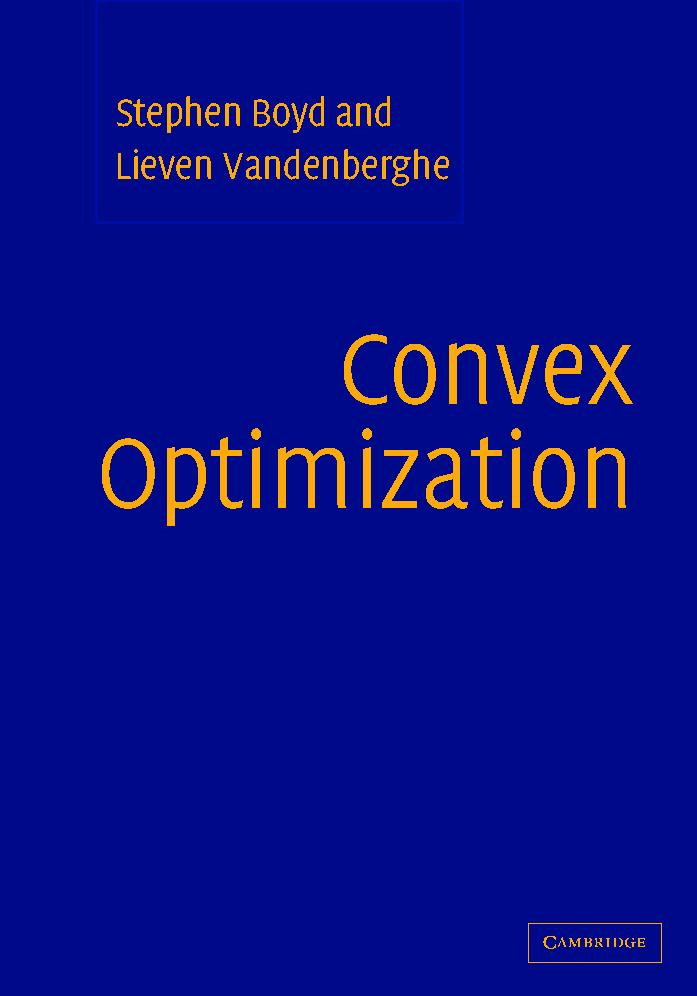
\includegraphics[height=0.6\textheight]{../Figures/convex-optimization/bv_cvxbook_cover}
\end{frame}
%
\begin{frame}{Level Sets and Sublevel Sets}

Let $f:\reals^{d}\to\reals$ be a function. Then we have the following
definitions:
\begin{definition}
A \textbf{level set} or \textbf{contour line} for the value $c$ is
the set of points $x\in\reals^{d}$ for which $f(x)=c$.
\end{definition}


\pause{}
\begin{definition}
A \textbf{sublevel} set for the value $c$ is the set of points $x\in\reals^{d}$
for which $f(x)\le c$.
\end{definition}


\pause{}
\begin{theorem}
If $f:\reals^{d}\to\reals$ is \textbf{convex}, then the \textbf{sublevel
sets are convex}. 
\end{theorem}


\pause{}

(Proof straight from definitions.)
\end{frame}
%
\begin{frame}{Convex Function}
\begin{center}
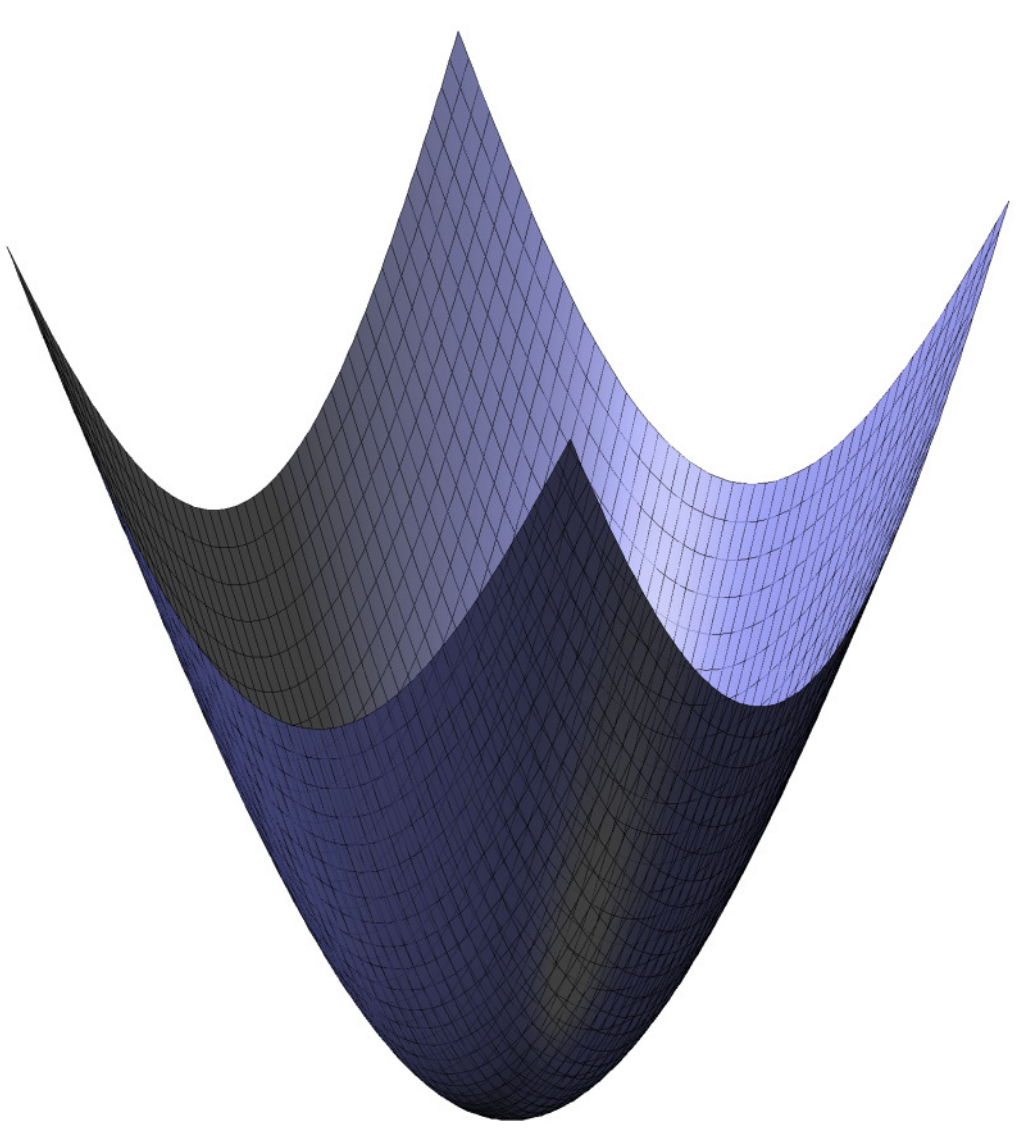
\includegraphics[height=0.65\textheight]{../Figures/subgradient-methods/3d-plot-convex-fn} 
\par\end{center}

\begin{center}
\let\thefootnote\relax\footnotetext{\tiny{Plot courtesy of Brett Bernstein.}}
\par\end{center}

\end{frame}
%
\begin{frame}{Contour Plot Convex Function: Sublevel Set}
\begin{center}
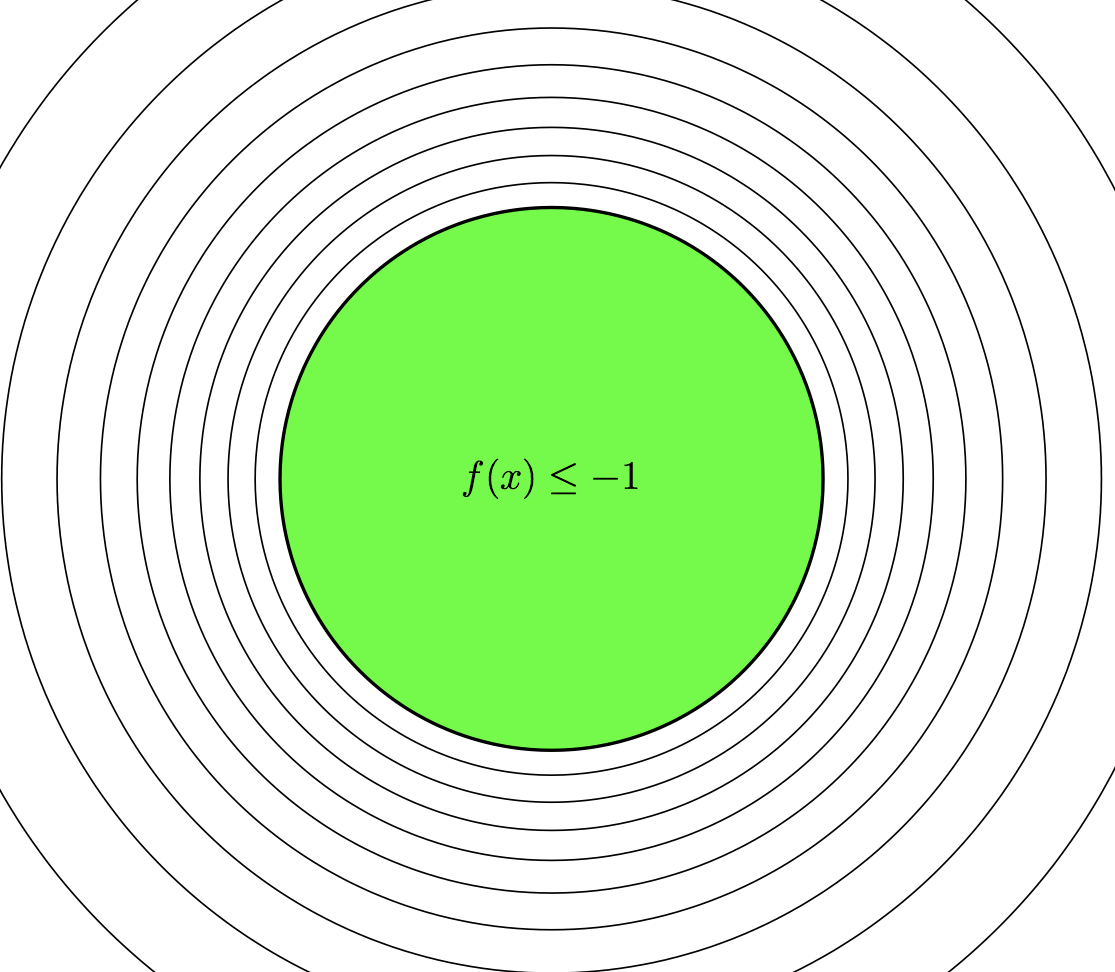
\includegraphics[height=0.65\textheight]{../Figures/subgradient-methods/contour-plot-convex-fn}
\par\end{center}

Is the sublevel set $\left\{ x\mid f(x)\le1\right\} $ convex?
\begin{center}
\let\thefootnote\relax\footnotetext{\tiny{Plot courtesy of Brett Bernstein.}}
\par\end{center}

\end{frame}
%
\begin{frame}{Nonconvex Function}
\begin{center}
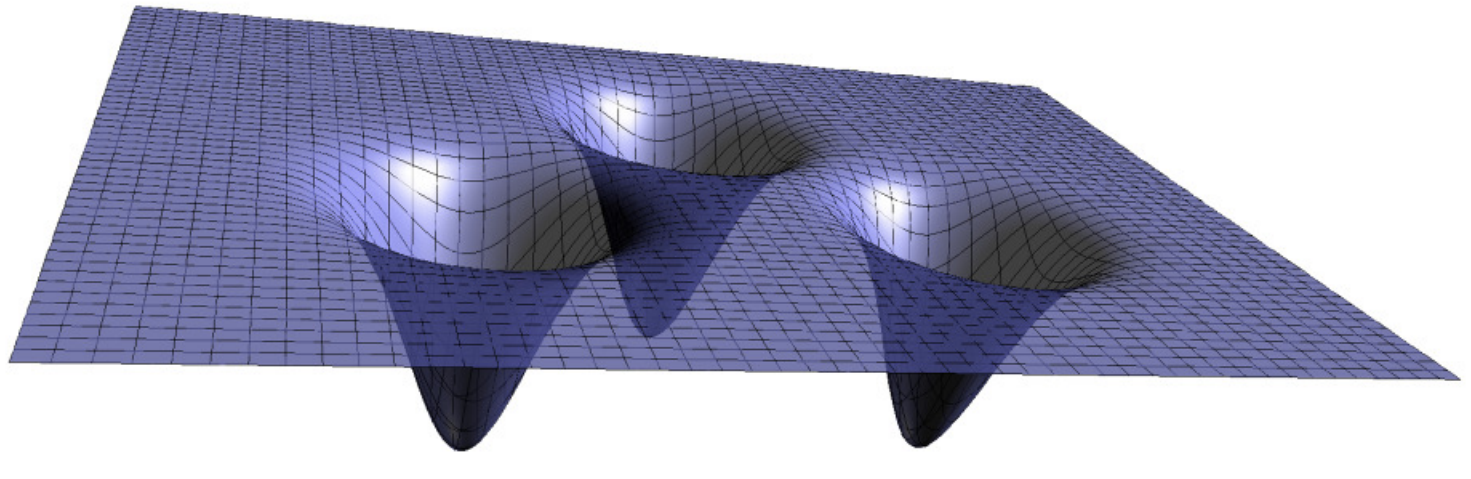
\includegraphics[height=0.7\textheight]{../Figures/subgradient-methods/3d-plot-nonconvex-fn}\let\thefootnote\relax\footnotetext{\tiny{Plot courtesy of Brett Bernstein.}}
\par\end{center}

\end{frame}
%
\begin{frame}{Contour Plot Nonconvex Function: Sublevel Set}
\begin{center}
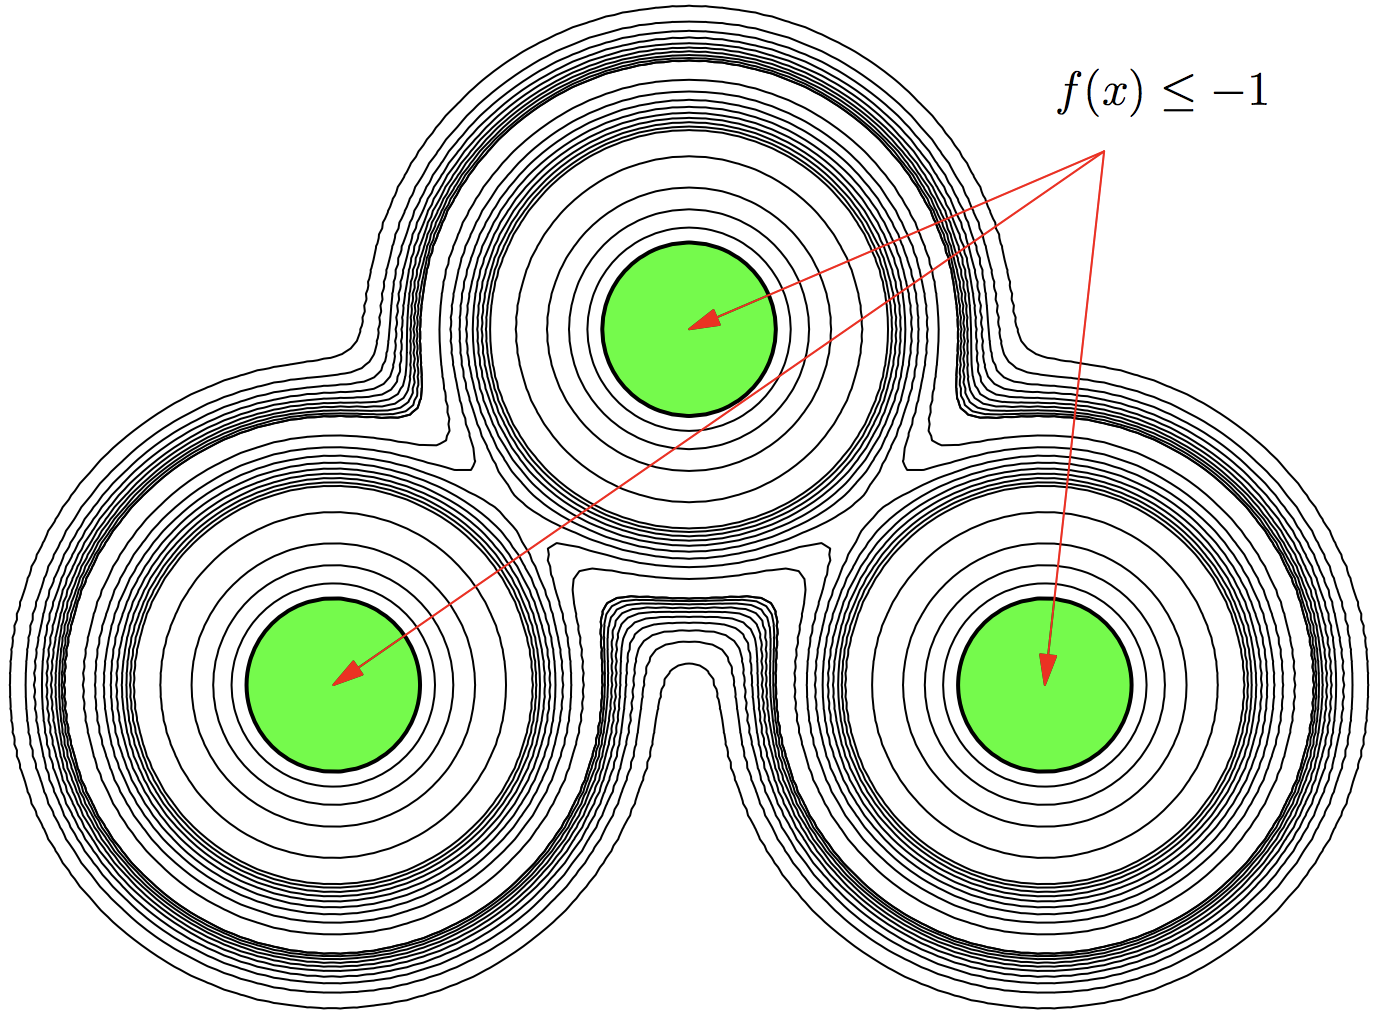
\includegraphics[height=0.65\textheight]{../Figures/subgradient-methods/contour-plot-nonconvex-fn}
\par\end{center}

Is the sublevel set $\left\{ x\mid f(x)\le1\right\} $ convex?
\begin{center}
\let\thefootnote\relax\footnotetext{\tiny{Plot courtesy of Brett Bernstein.}}
\par\end{center}

\end{frame}
%
\begin{frame}{Fact: Intersection of Convex Sets is Convex}
\begin{center}
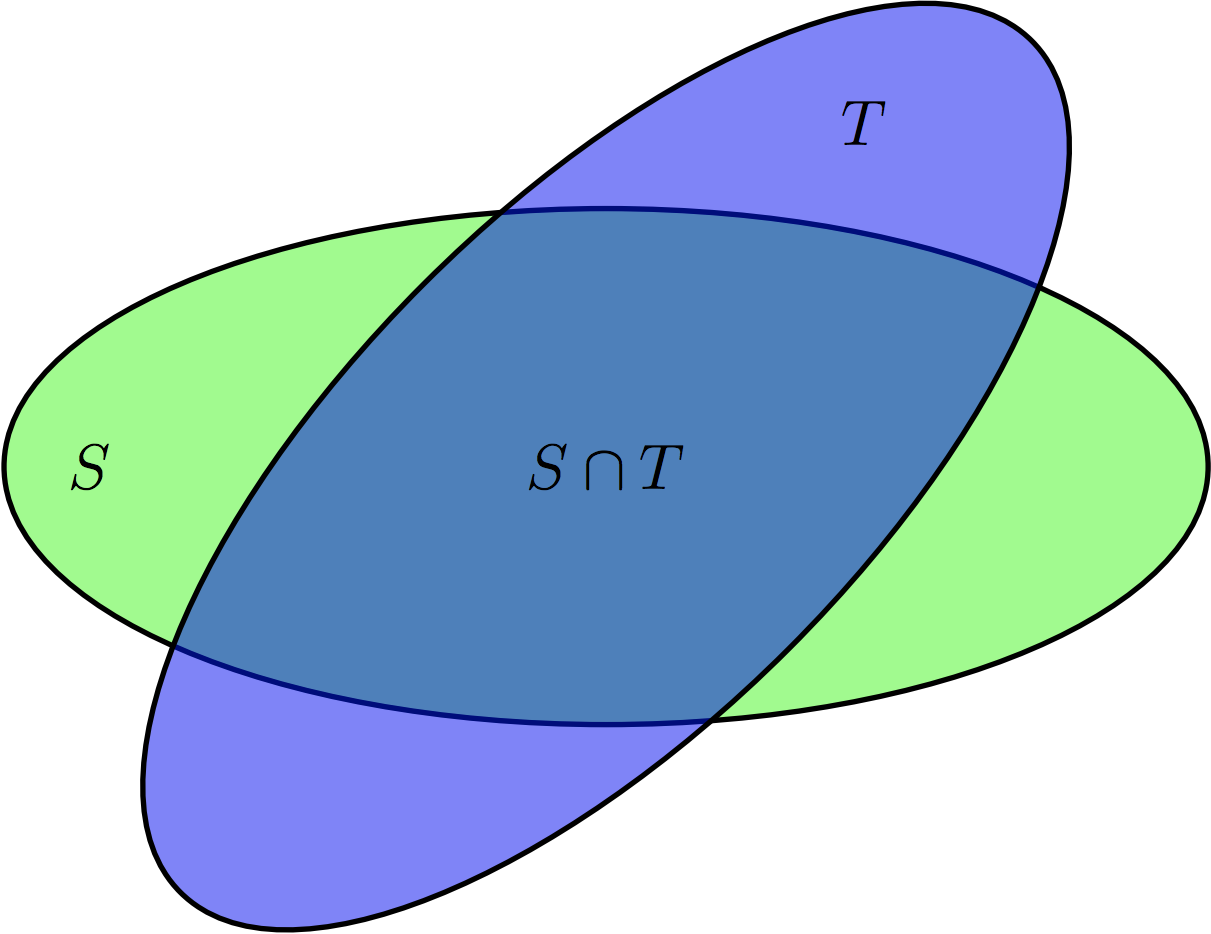
\includegraphics[height=0.65\textheight]{../Figures/subgradient-methods/convex-set-intersection} 
\par\end{center}

\begin{center}
\let\thefootnote\relax\footnotetext{\tiny{Plot courtesy of Brett Bernstein.}}
\par\end{center}

\end{frame}
%
\begin{frame}{Level and Superlevel Sets}
\begin{center}
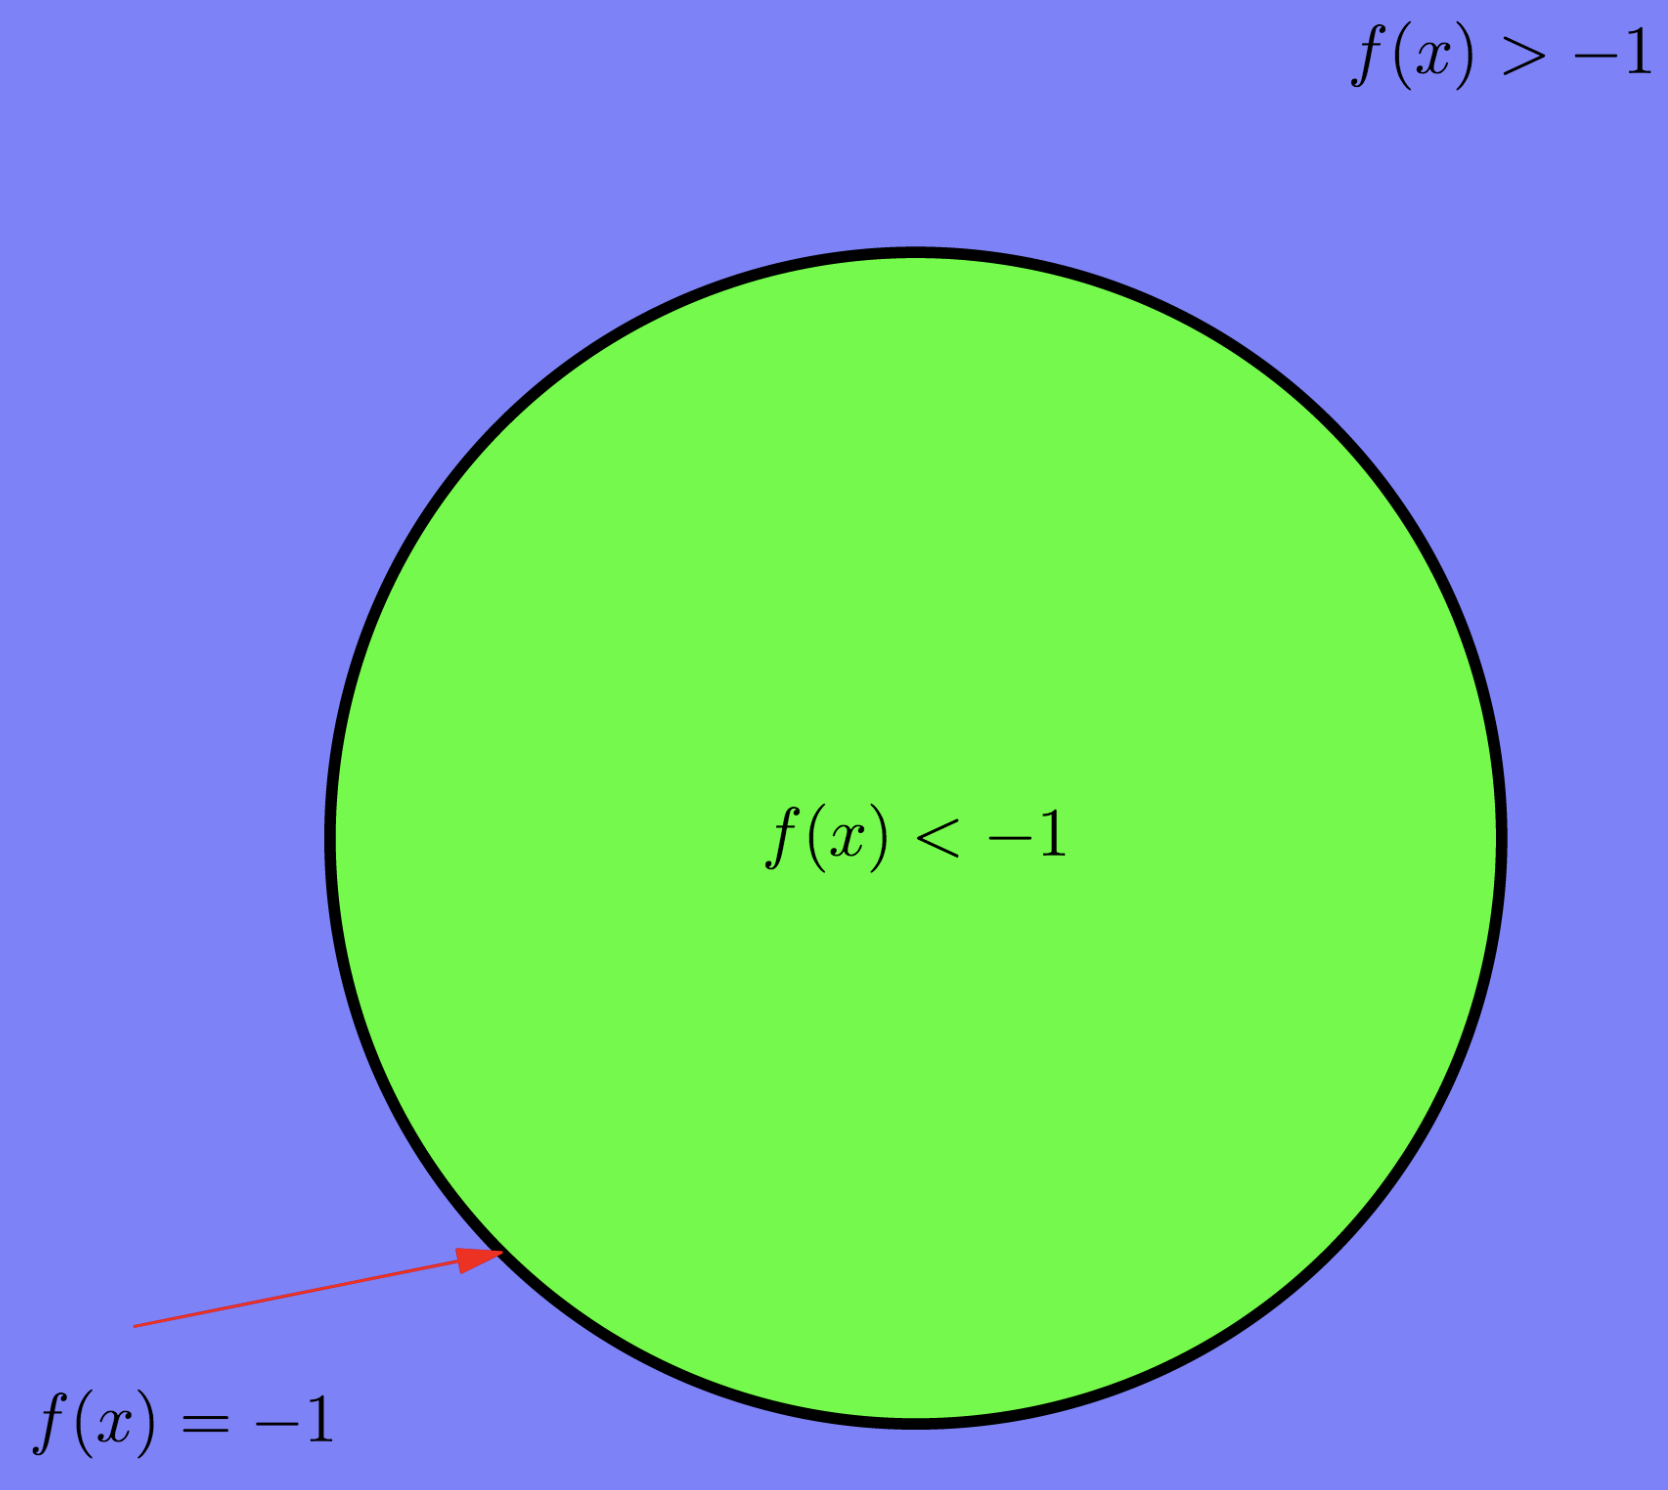
\includegraphics[height=0.65\textheight]{../Figures/subgradient-methods/superlevel-sets}
\par\end{center}

Level sets and superlevel sets of convex functions are \textbf{not}
generally convex.
\begin{center}
\let\thefootnote\relax\footnotetext{\tiny{Plot courtesy of Brett Bernstein.}}
\par\end{center}

\end{frame}
%
\begin{frame}{Convex Optimization Problem: Standard Form}
\begin{block}{Convex Optimization Problem: Standard Form}
\begin{eqnarray*}
\textrm{minimize} &  & f_{0}(x)\\
\textrm{subject to} &  & f_{i}(x)\le0,\;\;i=1,\ldots,m
\end{eqnarray*}
where $f_{0},\ldots,f_{m}$ are convex functions. 
\end{block}

\pause{}
\begin{itemize}
\item What can we say about each constraint set $\left\{ x\mid f_{i}(x)\le0\right\} ?\pause$
(convex)
\item What can we say about the feasible set $\left\{ x\mid f_{i}(x)\le0,\,i=1,\ldots,m\right\} ?\pause$
(convex)
\end{itemize}
\end{frame}
%
\begin{frame}{Convex Optimization Problem: Implicit Form}
\begin{block}{Convex Optimization Problem: Implicit Form}
\begin{eqnarray*}
\textrm{minimize} &  & f(x)\\
\textrm{subject to} &  & x\in C
\end{eqnarray*}
where $f$ is a convex function and $C$ is a convex set.

\pause{}

An alternative ``generic'' convex optimization problem.
\end{block}
\end{frame}
%

\section{Convex and Differentiable Functions}
\begin{frame}{First-Order Approximation}
\begin{itemize}
\item Suppose $f:\reals^{d}\to\reals$ is \textbf{differentiable.}
\item Predict $f(y)$ given $f(x)$ and $\del f(x)$?

\pause{}
\item Linear (i.e. ``\textbf{first order}'') approximation:
\[
f(y)\approx f(x)+\del f(x)^{T}(y-x)
\]
\end{itemize}
\begin{center}
\let\thefootnote\relax\footnotetext{\tiny{Boyd \& Vandenberghe Fig. 3.2}}
\par\end{center}

\begin{center}
\includegraphics[width=0.7\columnwidth]{../Figures/convex-optimization/BVFig3\lyxdot 2-convexTangent}
\par\end{center}

\end{frame}
%
\begin{frame}{First-Order Condition for Convex, Differentiable Function}

\begin{itemize}
\item Suppose $f:\reals^{d}\to\reals$ is \textbf{convex} and \textbf{differentiable.}
\item Then for any $x,y\in\reals^{d}$
\[
f(y)\ge f(x)+\del f(x)^{T}(y-x)
\]


\pause{}
\item The linear approximation to $f$ at $x$ is a \textbf{global underestimator
}of $f$:
\end{itemize}
\let\thefootnote\relax\footnotetext{\tiny{Figure from Boyd \& Vandenberghe Fig. 3.2; Proof in Section 3.1.3 }}
\begin{center}
\includegraphics[width=0.7\columnwidth]{../Figures/convex-optimization/BVFig3\lyxdot 2-convexTangent}
\par\end{center}

\end{frame}
%
\begin{frame}{First-Order Condition for Convex, Differentiable Function}
\begin{itemize}
\item Suppose $f:\reals^{d}\to\reals$ is \textbf{convex} and \textbf{differentiable}
\item Then for any $x,y\in\reals^{d}$
\[
f(y)\ge f(x)+\del f(x)^{T}(y-x)
\]


\pause{}

\end{itemize}
\begin{corollary}
If $\del f(x)=0$ then $x$ is a global minimizer of $f$.
\end{corollary}


\pause{}

For convex functions, \textbf{local information gives global information.}
\end{frame}

\section{Subgradients }
\begin{frame}{Subgradients}
\begin{definition}
A vector $g\in\reals^{d}$ is a \textbf{subgradient} of $f:\reals^{d}\to\reals$
at $x$ if for all $z$, 
\[
f(z)\ge f(x)+g^{T}(z-x).
\]

\pause{}
\end{definition}

\begin{center}
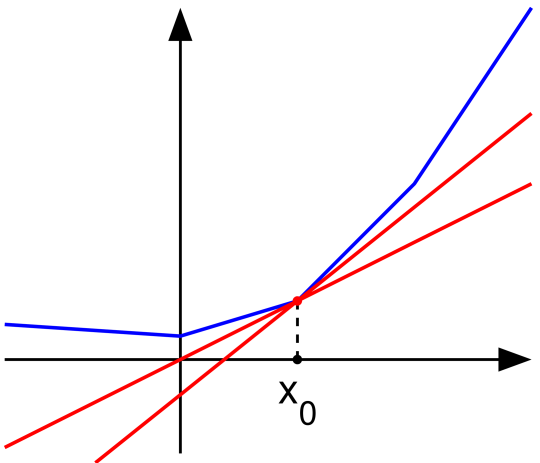
\includegraphics[height=0.4\textheight]{../Figures/convex-optimization/Subderivative_illustration}
\par\end{center}

Blue is a graph of $f(x)$. \\
Each red line $x\mapsto f(x_{0})+g^{T}\left(x-x_{0}\right)$ is a
global lower bound on $f(x)$.
\end{frame}
%
\begin{frame}{Subdifferential}
\begin{definitions}
\begin{itemize}
\item $f$ is \textbf{subdifferentiable} at $x$ if $\exists$ at least
one subgradient at $x$. 
\item The set of all subgradients at $x$ is called the \textbf{subdifferential:}
$\partial f(x)$ 

\pause{}

\end{itemize}
\end{definitions}

\begin{block}{Basic Facts}
\end{block}
\begin{itemize}
\item $f$ is convex and differentiable $\implies$ $\partial f(x)=\left\{ \del f(x)\right\} $.

\pause{}
\item Any point $x$, there can be $0$, $1$, or infinitely many subgradients.

\pause{}
\item $\partial f(x)=\emptyset$ $\implies$ $f$ is not convex.
\end{itemize}
\end{frame}

\begin{frame}{Globla Optimality Condition}
\begin{definition}
A vector $g\in\reals^{d}$ is a \textbf{subgradient} of $f:\reals^{d}\to\reals$
at $x$ if for all $z$, 
\[
f(z)\ge f(x)+g^{T}(z-x).
\]

\pause{}

\end{definition}

\begin{corollary}
If $0\in\partial f(x)$, then $x$ is a \textbf{global minimizer}
of $f$.
\end{corollary}

\end{frame}

\begin{frame}{Subdifferential of Absolute Value}
\begin{itemize}
\item Consider $f(x)=\left|x\right|$

\pause{}

\end{itemize}
\let\thefootnote\relax\footnotetext{\tiny{Boyd EE364b: Subgradients Slides}}

\begin{center}
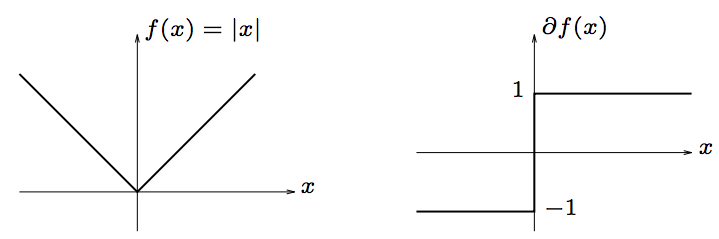
\includegraphics[width=0.8\columnwidth]{../Figures/convex-optimization/subgradient-absolute-value}
\par\end{center}
\begin{itemize}
\item Plot on right shows $\left\{ (x,g)\mid x\in\reals,\;g\in\partial f(x)\right\} $ 
\end{itemize}
\end{frame}
%
\begin{frame}{$f(x_{1},x_{2})=\left|x_{1}\right|+2\left|x_{2}\right|$}
\begin{center}
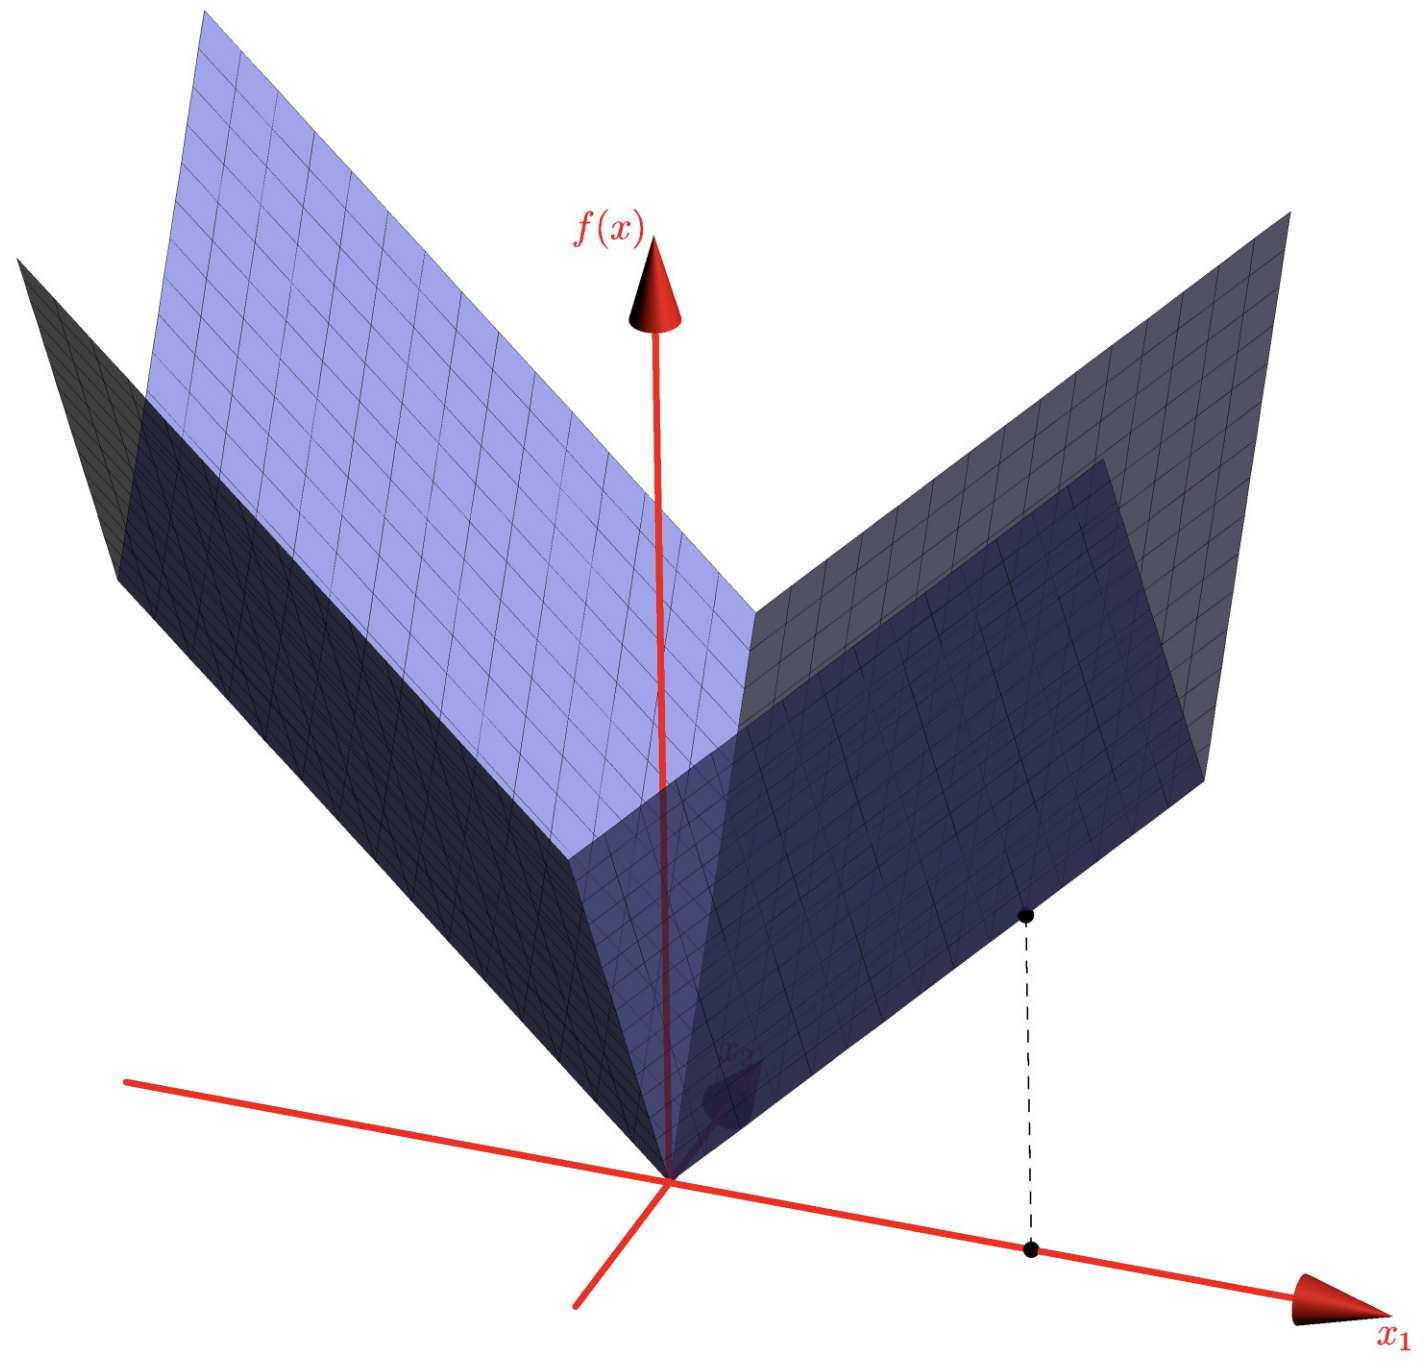
\includegraphics[height=0.75\textheight]{../Figures/subgradient-methods/3d-plot-abs-x1-plus-2absx2}\let\thefootnote\relax\footnotetext{\tiny{Plot courtesy of Brett Bernstein.}}
\par\end{center}

\end{frame}
%
\begin{frame}{Subgradients of $f(x_{1},x_{2})=\left|x_{1}\right|+2\left|x_{2}\right|$}
\begin{itemize}
\item Let's find the subdifferential of $f(x_{1},x_{2})=\left|x_{1}\right|+2\left|x_{2}\right|$
at $\left(3,0\right)$.
\end{itemize}

\pause{}
\begin{itemize}
\item First coordinate of subgradient must be $1$, from $\left|x_{1}\right|$
part (at $x_{1}=3$).
\end{itemize}

\pause{}
\begin{itemize}
\item Second coordinate of subgradient can be anything in $\left[-2,2\right]$.
\end{itemize}

\pause{}
\begin{itemize}
\item So graph of $h(x_{1},x_{2})=f(3,0)+g^{T}\left(x_{1}-3,x_{2}-0\right)$
is a global underestimate of $f(x_{1},x_{2})$, for any $g=\left(g_{1},g_{2}\right),$
where $g_{1}=1$ and $g_{2}\in[-2,2]$. 
\end{itemize}
\end{frame}
%
\begin{frame}{Underestimating Hyperplane to $f(x_{1},x_{2})=\left|x_{1}\right|+2\left|x_{2}\right|$}
\begin{center}
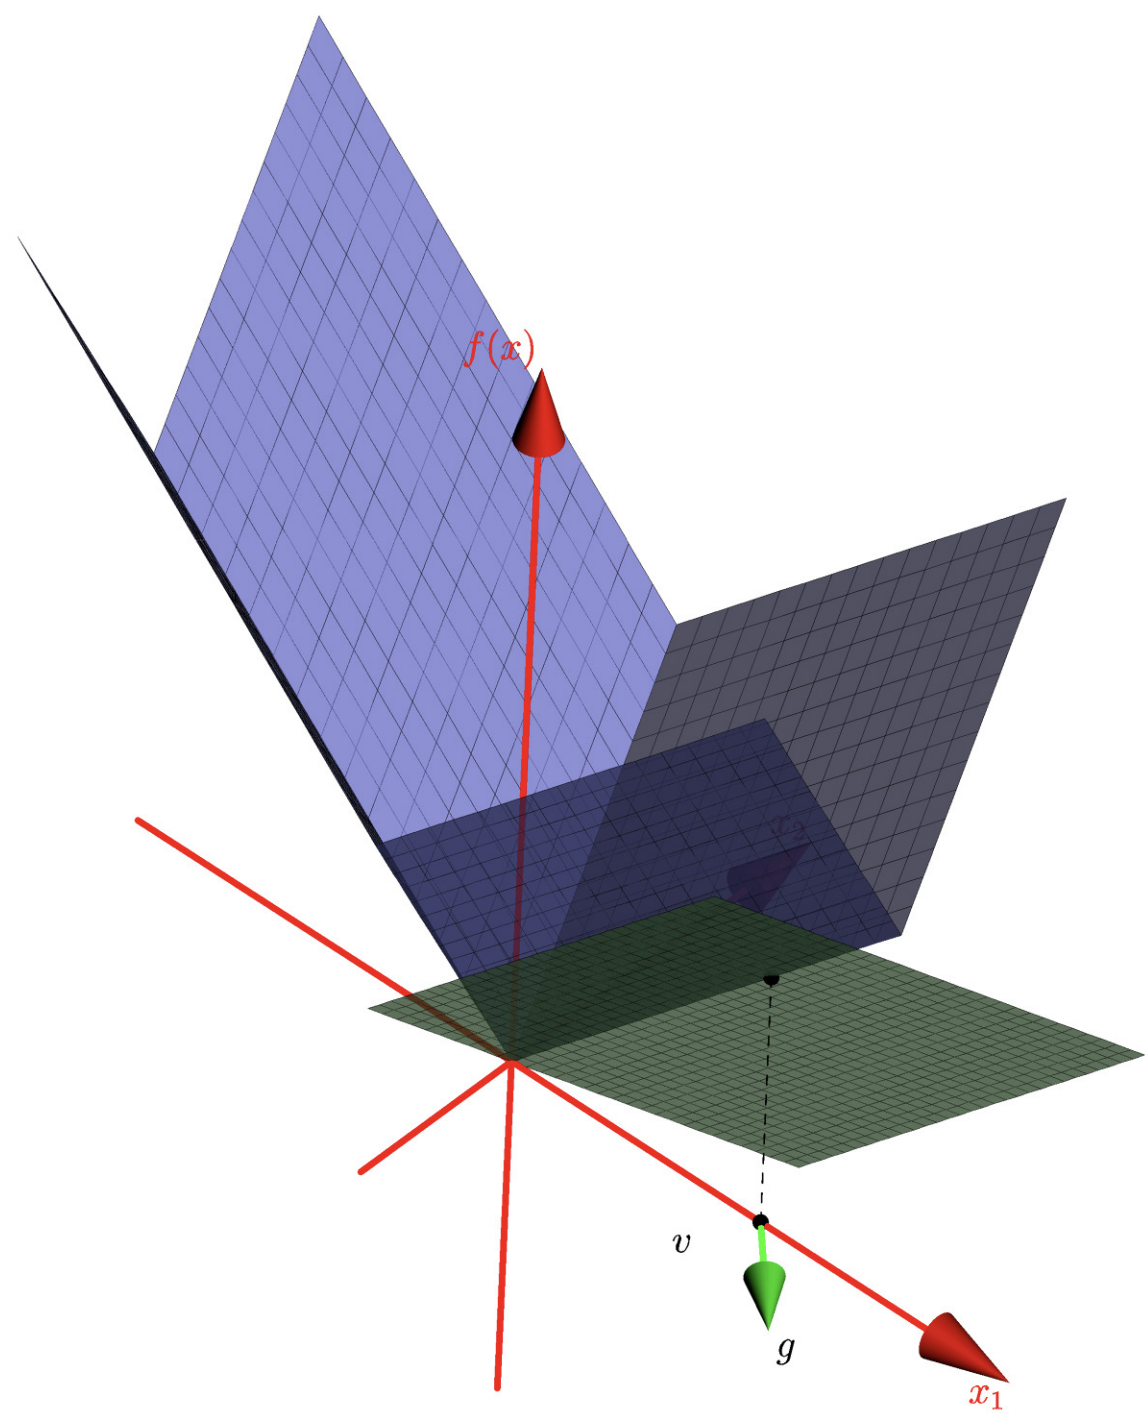
\includegraphics[height=0.75\textheight]{../Figures/subgradient-methods/underestimating-3d-plot-abs-x1-plus-2absx2}\let\thefootnote\relax\footnotetext{\tiny{Plot courtesy of Brett Bernstein.}} 
\par\end{center}

\end{frame}

\begin{frame}{Important Properties of Subdifferential}
\begin{itemize}
\item If $f_1,\dots,f_m:\reals^d \rightarrow \reals$ are convex functions and $f = f_1+\cdots + f_m$, then $\partial f(x) = \partial f_1(x) + \cdots +\partial f_m(x)$.
\item For $\alpha \geq 0$, $\partial (\alpha f) (x) = \alpha \partial f(x)$. 	
\end{itemize}
	
\end{frame}

\begin{frame}{Subgradients of $f(x) = \|x\|_1$}
\begin{itemize}
\item Let's find the subdifferential of $f(x) = \|x\|_1 = \sum_{i=1}^d |x_i|$ at any given point $x^0 = (x^0_1,x^0_2, \dots, x^0_d)$.
\item By an important property of subdifferential: If $f = f_1+\cdots+f_m$, then $\partial f(x) = \partial f_1(x) + \cdots \partial f_m(x)$. 
\item We could calculate the subgradient of $f^i(x) = |x_i|$ and sum them up.
\item The subgradient $g^i = (g^i_1,\dots, g^i_d)$ of $f^i(x) = |x_i|$ at $x^0 = (x^0_1,x^0_2, \dots, x^0_d)$ is:
\[
g_j^i = 0, \quad {j\neq i}; \quad g_j^i = s(x^0_j), \quad j = i,
\]
where $s(x) = \text{sign}(x)$ if $x\neq 0$ and $s(x) \in [-1,1]$ if $x = 0$
\item We sum all the $g^i$ up to get the subgradient $g = (g_1,\dots, g_d)$ of $f(x)$ at $x^0$:
\[
g_i = s(x^0_i) \quad \text{for all } i
\]
\end{itemize}

\end{frame}

%

\section{Subgradient Descent}
\begin{frame}{Subgradient Descent}
\begin{itemize}
\item Suppose $f$ is convex, and we start optimizing at $x_{0}$.
\item Repeat
\begin{itemize}
\item Step in a negative subgradient direction: 
\[
x=x_{0}-tg,
\]
where $t>0$ is the step size and $g\in\partial f(x_{0})$.
\end{itemize}
\end{itemize}

\pause{}
\begin{itemize}
\item $-g$ not a descent direction -- can this work?
\end{itemize}
\end{frame}

\begin{frame}{Convergence Theorem for Fixed Step Size}

Assume $f:\reals^{n}\to\reals$ is convex and
\begin{itemize}
\item $f$ is Lipschitz continuous with constant $G>0$:
\[
\left|f(x)-f(y)\right|\le G\|x-y\|\mbox{ for all }x,y
\]
\end{itemize}
\begin{theorem}
For fixed step size $t$, subgradient method satisfies:
\[
\lim_{k\to\infty}f(x_{\text{best}}^{(k)})\le f(x^{*})+G^{2}t/2
\]
\end{theorem}

\begin{center}
\let\thefootnote\relax\footnotetext{\tiny{Based on \url{https://www.cs.cmu.edu/~ggordon/10725-F12/slides/06-sg-method.pdf}}}
\par\end{center}

\end{frame}

\begin{frame}{Convergence Theorems for Decreasing Step Sizes}

Assume $f:\reals^{n}\to\reals$ is convex and
\begin{itemize}
\item $f$ is Lipschitz continuous with constant $G>0$:
\[
\left|f(x)-f(y)\right|\le G\|x-y\|\mbox{ for all }x,y
\]
\end{itemize}
\begin{theorem}
For step size respecting Robbins-Monro conditions,
\[
\lim_{k\to\infty}f(x_{\text{best}}^{(k)})=f(x^{*})
\]
\end{theorem}

\begin{center}
\let\thefootnote\relax\footnotetext{\tiny{Based on \url{https://www.cs.cmu.edu/~ggordon/10725-F12/slides/06-sg-method.pdf}}}
\par\end{center}
\end{frame}

\begin{frame}{Subgradient Descent for Lasso Problem}
\begin{itemize}
\item Lasso problem can be parametrized as
\[
\min_{w\in\reals^{d}}J(w) = \frac{1}{n}\sum_{i=1}^{n}\left\{ w^{T}x_{i}-y_{i}\right\} ^{2}+\lambda\|w\|_{1}
\]
\pause{}
\item Subgradients of $J(w)$ are
\[
\frac{1}{n}\sum_{i=1}^n 2\{w^Tx_i-y_i\}x_i+\lambda s,
\]
where $s_i = \text{sign}(w_i)$ if $w_i\neq 0$ and $s_i \in [-1,1]$ if $w_i=0$.
\end{itemize}
\end{frame}

\begin{frame}{Subgradient Descent for Lasso Problem: Potential Issues}
\begin{itemize}
\item Subgradient descent will work for all convex and Lipschitz continuous objective functions.
\pause{}
\item BUT, convergence can be very \textbf{slow} for non-differentiable functions
\pause{}
\item One can often find better approaches by closer examination of the objective function. For example, shooting method or projected SGD.
\pause{}
\item Taking small steps in the direction of the (sub)gradient usually may \textbf{not} lead to zero coordinates.
\pause{}
\item BUT, in practice, we can threshold small values.
\end{itemize}
	
\end{frame}
\begin{frame}{Appendix: Subgradient Gets Us Closer To Minimizer}
\begin{theorem}
Suppose $f$ is convex.
\begin{itemize}
\item Let $x=x_{0}-tg$, for $g\in\partial f(x_{0})$.
\item Let $z$ be any point for which $f(z)<f(x_{0})$.
\item Then for small enough $t>0$,
\[
\|x-z\|_{2}<\|x_{0}-z\|_{2}.
\]
\end{itemize}

\pause{}
\end{theorem}

\begin{itemize}
\item Apply this with $z=x^{*}\in\argmin_{x}f(x)$. 
\end{itemize}
$\implies$\textbf{Appendix: Negative subgradient step gets us closer to minimizer}.
\end{frame}

\begin{frame}{Subgradient Gets Us Closer To Minimizer (Proof)}
\begin{itemize}
\item Let $x=x_{0}-tg$, for $g\in\partial f(x_{0})$ and $t>0$.
\item Let $z$ be any point for which $f(z)<f(x_{0})$.
\item Then
\begin{eqnarray*}
\|x-z\|_{2}^{2} & = & \|x_{0}-tg-z\|_{2}^{2}\\
\pause & = & \|x_{0}-z\|_{2}^{2}-2tg^{T}\left(x_{0}-z\right)+t^{2}\|g\|_{2}^{2}\\
\pause & \le & \|x_{0}-z\|_{2}^{2}-2t\left[f(x_{0})-f(z)\right]+t^{2}\|g\|_{2}^{2}
\end{eqnarray*}


\pause{}
\item Consider $-2t\left[f(x_{0})-f(z)\right]+t^{2}\|g\|_{2}^{2}$. 
\begin{itemize}
\item It's a convex quadratic (facing upwards).
\item Has zeros at $t=0$ and $t=2\left(f(x_{0})-f(z)\right)/\|g\|_{2}^{2}>0$.
\item Therefore, it's negative for any 
\[
t\in\left(0,\frac{2\left(f(x_{0})-f(z)\right)}{\|g\|_{2}^{2}}\right).
\]
\end{itemize}

\let\thefootnote\relax\footnotetext{\tiny{Based on Boyd EE364b: Subgradients Slides}}
\end{itemize}
\end{frame}

\end{document}
